%%%%%%%%%%%%%%%%%%%%%%%%%%%%%% -*- Mode: Latex -*- %%%%%%%%%%%%%%%%%%%%%%%%%%%%
%% 04-14-system.tex -- Thesis Proposal - PRI
%% Author          : Aaron A. Kagawa
%% Created On      : Mon Sep 23 11:52:28 2004
%% Last Modified By: Aaron Kagawa
%% Last Modified On: Tue Feb  8 21:20:54 2005
%% RCS: $Id$
%%%%%%%%%%%%%%%%%%%%%%%%%%%%%%%%%%%%%%%%%%%%%%%%%%%%%%%%%%%%%%%%%%%%%%%%%%%%%%
%%   Copyright (C) 2004 Aaron A. Kagawa
%%%%%%%%%%%%%%%%%%%%%%%%%%%%%%%%%%%%%%%%%%%%%%%%%%%%%%%%%%%%%%%%%%%%%%%%%%%%%%%

\chapter{Hackystat Priority Ranked Inspection Extension}
\label{chapter:system}
This chapter provides a detailed description of the Hackystat PRI
(hackyPRI) extension. hackyPRI extends the functionality of the Hackystat
system to provide the PRI determination of more and less in need of
inspection (MINI and LINI). I will discuss how hackyPRI supports the four
steps of the Priority Ranked Inspection process.

%%Next, I will provide a detailed description of the design and
%%implementation of the hackyPRI extension.

\section{The Four Steps of the Priority Ranked Inspection Process}
Hackystat PRI Extension supports the four steps of the Priority Ranked
Inspection process. The following list is the four steps of the PRI
process.

\begin{enumerate}
\item The creation of the PRI weighting function, which distinguishes MINI
  documents from LINI documents. The weighting function design includes two 
  steps: 
\begin{enumerate}
\item Selection of product and process measures to use in the PRI
  weighting function.
\item Creation of a numerical weighting system that assigns a weight for
  each measure and the calibration of this weighting system.
\end{enumerate}
\item The selection of a document for inspection based on the PRI
  weighting function and ranking.
\item The actual inspection of the selected document.
\item Adjustment of product and process measure selection and
  calibration based on the results of the inspection.
\end{enumerate}

The following subsections detail how hackyPRI supports the steps.

\subsection{Step 1a: Selection of Product and Process Measures}
The Hackystat system provides a set of Sensor Data Types that represent
various software product and process measures. I will use a subset of the
available Sensor Data Types as the measures that make up the PRI weighting
function. Table \ref{table:measures-hackyPRI} contains a description of the
measures that will be used in the hackyPRI extension.

\begin{table}[htbp]
  \begin{center}
    \caption{Measures used in hackyPRI}
    \label{table:measures-hackyPRI}
    \begin{tabular}{|p{3.0cm}|p{10.0cm}|} \hline
      {\bf Measure} & {\bf Description} \\ \hline
\small{}Expert & \small{}The developer who has the most active time and
commits. An expert represents the developer who is most familiar with the
particular portion of the system. \\ \hline

\small{}Active Time & \small{}The total time developers spent editing a
particular file. This measure is obtainable from attaching Hackystat
sensors to the developers' Integrated Developer Environment (i.e., Emacs,
JBuilder, Eclipse) \\ \hline
\small{}Last Active Time & \small{}The day of the last active time. \\ \hline
\small{}\# of Developer \newline Active Time \newline Contributions &
\small{}The number of unique developers who have contributed to the total
active time. \\ \hline

\small{}Commits & \small{}The total number of commits to a particular
file. This measure is obtainable from attaching Hackystat sensors to a
Concurrent Version Control server (i.e., CVS). \\ \hline
\small{}Last Commit & \small{}The day of the last commit. \\ \hline
\small{}\# of Developer \newline Commit \newline Contributions &
\small{}The number of unique developers who have contributed to the total
commits. \\ \hline

\small{}Review & \small{}The number of code reviews (inspections) that were
conducted. This measure is obtainable from attaching Hackystat sensors
to the Eclipse Jupiter Review plugin.\\ \hline
\small{}Last Review & \small{}The day of the last review or inspection. \\ \hline  

\small{}Defects & \small{}The number of defects that were reported and
stored in the Defect Tracking tool. This measure is obtainable from
attaching Hackystat sensors to the Jira tool.\\ \hline
\small{}Last Defect & \small{}The day of the last defect. \\ \hline

\small{}Enhancements & \small{}The number of enhancements that are
requested. This measure is obtainable from attaching Hackystat sensors to
the Jira tool.\\ \hline
\small{}Last Enhancement & \small{}The day of the last enhancement. \\ \hline

\small{}File Metrics & \small{}The last known metrics of non-test code;
lines of code, number of methods, and number of classes. This measure is
obtainable from attaching Hackystat sensors to the LOCC tool. \\ \hline
\small{}Test File Metrics & \small{}The lines of test code, number of test
methods, and the number of test classes. This measure is obtainable from
the Hackystat sensors to the LOCC tool. \\ \hline

\small{}Dependency & \small{}The inbound and outbound references that
indicate dependencies within the system. This measure is obtainable
from attaching Hackystat sensors to the DependencyFinder tool.\\ \hline

\small{}Unit Tests & \small{}The number of unit tests that are executed
during the last build of the system. This measure is obtainable from
attaching Hackystat sensors to the JUnit tool. \\ \hline 

\small{}Test Failures & \small{}The total number of test failures. This
measure is obtainable from attaching Hackystat sensors to the JUnit
tool. \\ \hline

\small{}Coverage & \small{}The last know coverage percentage of the
system. This measure represents the number of methods that are executed
during a test invocation over the number of total methods. This measure is
obtainable from attaching Hackystat sensors to the JBlanket tool.. \\ \hline

    \end{tabular}
  \end{center}
\end{table}

Each measure is collected for each package or workspace within a specified
project. Figure \ref{fig:WorkspaceQualityAnalysis} shows several example
LINI packages.

\begin{figure*}[ht]
  \centering
  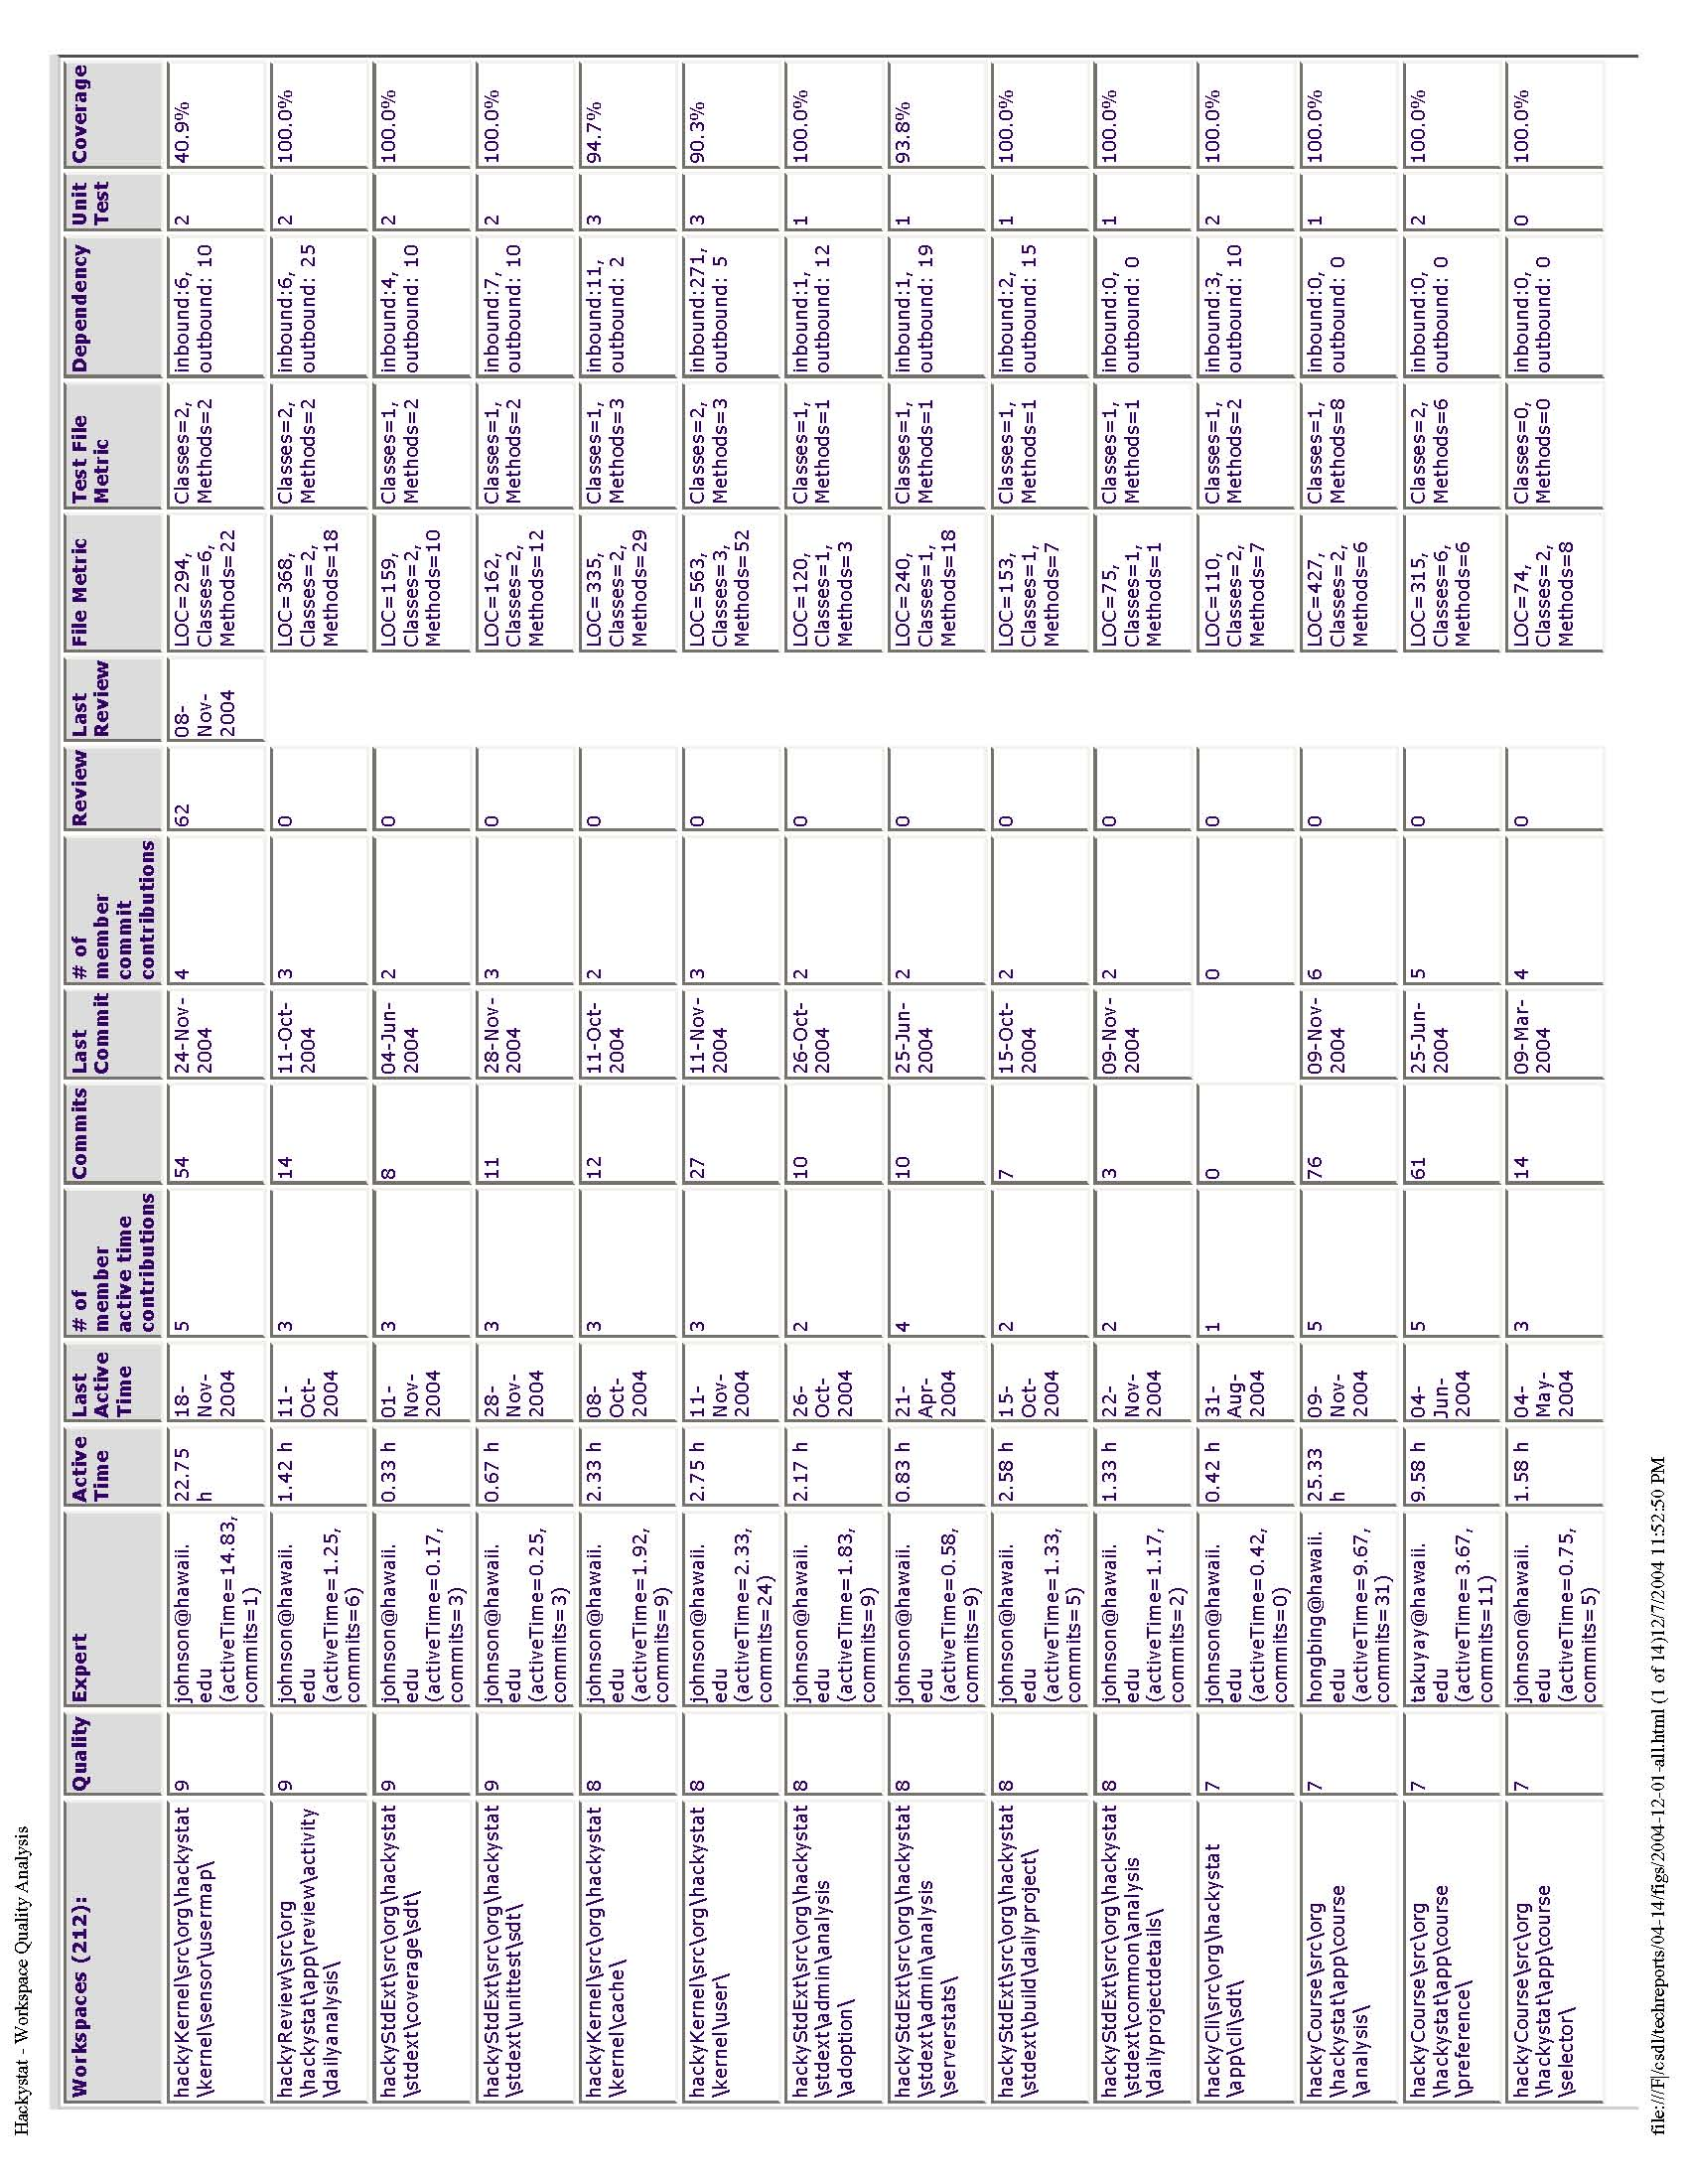
\includegraphics[width=1.00\textwidth]{figs/2004-12-01-all_Page_01.eps}
  \caption{The Workspace PRI analysis. Workspaces are listed with its
  respective PRI ranking and the measures.
}
  \label{fig:WorkspaceQualityAnalysis}
\end{figure*}


\subsection{Step 1b: Calibration of Product and Process Measures}
Each measure and its numerical weight will be stored within the hackyPRI
extension. The numerical weights are not shown in Figure
\ref{fig:WorkspaceQualityAnalysis}, however the calibration and weighting
system works behind the scenes. 

To make the important distinction of MINI and LINI, I assign certain
numerical weights to the measures. For example, if the coverage of a
package is below 80 percent, I assign a ``low'' weight for that measure. If
the coverage of a package is a 100 percent, then I assign a ``high''
weight. ``Low'' is operationalized by a 1, ``high'' is operationalized by a
3, and ``middle ground'' is operationalized by a 2. The system assigns each
measure a weight after analyzing its value. Table
\ref{table:weighting-hackyPRI} contains a description of the weighting used
in the hackyPRI extension.

After all measures are assigned a weight, the weights are aggregated to
provide a combined weight for each package. The packages are then ranked by
the packages' aggregate PRI level, sorting the MINI packages to the bottom
and LINI packages to the top.

\begin{table}[htbp]
  \begin{center}
    \caption{The Weighting System used in hackyPRI}
    \label{table:weighting-hackyPRI}
    \begin{tabular}{|p{2.5cm}|p{3.0cm}|p{8.0cm}|} \hline
      {\bf Measure} & {\bf Weighting} & {\bf Discussion} \\ \hline
\small{}Expert & \small{}johnson=3 \newline anyone else=1 &
\small{}Dr. Johnson is an active Hackystat developer. He is the most
experienced programmer in CSDL. In addition, a lot of his development are
technical over passes of the code to ensure that the code is of high
quality. Therefore, code that he develops is weighted higher than
others. \\ \hline

\small{}Active Time & \small{}Not Weighted  &  \\ \hline
\small{}Last Active Time & \small{}Not Weighted & \\ \hline
\small{}\# of Developer \newline Active Time \newline Contributions & 
\small{}3+ developers=2 \newline 2 developers=1 \newline 1 developer=0
\newline none=0 & \small{}If code has been developed solely by one
person, the code is more likely to contain defects. As more developers work 
on the code, the less likely defects will occur. \\ \hline

\small{}Commits & \small{}Not Weighted & \\ \hline
\small{}Last Commit & \small{}Not Weighted & \\ \hline
\small{}\# of Developer \newline Commit \newline Contributions & \small{} 
\small{}3+ developers=2 \newline 2 developers=1 \newline 1 developer=0 &
\small{}Commit data is another way to determine if developers are working
on a particular piece of code. If code has been developed solely by one
person, the code is more likely to contain defects. As more developers work
on the code, the less likely defects will occur. \\ \hline

\small{}Review & \small{}2+ reviews=2 \newline 1 review=1 \newline none=0 & 
More reviews (inspections) that are conducted equals higher quality code. \\ \hline
\small{}Last Review & \small{}today-last$>$30=2 \newline today-last$<$31=1
\newline none=0 & \small{}Code that has been reviewed recently tends to be
higher quality code. \\ \hline 

\small{}Defects & \small{}Not Weighted & \small{}In development \\ \hline
\small{}Last Defect & \small{}Not Weighted & \small{}In development \\ \hline

\small{}File Metrics & \small{}Not Weighted & \small{} \\ \hline
\small{}Test File Metrics & \small{}Not Weighted  & \small{} \\ \hline

\small{}Dependency & \small{}1=inbound$>$outbound & \small{}Inbound
references represents the number of references that use a specific
class. Outbound represents the number of references that the class
uses. The more inbound references the more likely changes in a class will
impact other classes.\\ \hline

\small{}Unit Test & \small{}$>$0=1 & \small{}Each day a set of unit tests
are executed against the system. If there is at least one or more
executions then we can be fairly certain that some portion of the system
was tested. However, this does not represent the effectiveness and
thoroughness of the tests. Effectiveness and thoroughness can be measured
with a combination of Test Failure, Coverage, and Defects.\\ \hline

\small{}Test Failures & \small{} & \small{} \\ \hline

\small{}Coverage & \small{}100\%=2 \newline 99-90+\%=1 \newline 89-0=\%=0 &
\small{}Higher coverage percentage, every thing else being equal,
translates to higher quality code. \\ \hline

    \end{tabular}
  \end{center}
\end{table}


There are several issues with the assignment of numerical weights that I
still need to address. For example, I explicitly determine the weights
using my own subjective measure of what is low versus high quality.  I will
need to explore if my subjective measure is sufficient, if some measures
should be weighted more than others, or if any other entirely different
weighting methods provide more accurate results.

\subsection{Step 2: Selecting a Document for Inspection Based on the PRI
  Ranking} Using the PRI Hackystat analysis, an organization should
select a document at the bottom of the PRI ranking table for inspection.
The higher the document is in the table, the less it is in need of
inspection. 

In my initial studies, I have found that simply picking the highest
priority document, or the document that is at the very bottom of the chart,
will probably not be the ``best'' document to inspect. In most cases, I
have found that the PRI ranking aids the selection of a document, but it
does not select the document for you. In other words, it is more useful to
consider a few documents from the bottom portion of the ranking and take an
educated guess as to which document needs inspection more.

\subsection{Step 3: Conducting an Inspection of the Selected Document}
Once a document is selected it can be inspected. One interesting side
effect of the PRI ranking is that specific statistics and measures can be
presented during the inspection process. For example, if a document is
selected because it has low coverage, then the inspection can focus on why
the coverage is low.

The Hackystat PRI Extension or the PRI process does not support the actual
inspection of the document. Instead, an organization should consult
traditional inspection processes (i.e., Software Inspection, Fagan
Inspection, In-Process Inspection, etc). In other words, the PRI process is
an outer layer that wraps around an already established inspection process.

\subsection{Step 4: Adjustment of the Measure Selection and Calibration}
If a document is shown to be incorrectly ranked, then an adjustment of the
PRI weighting function is necessary. In hackyPRI this can be accomplished
by adding more Hackystat measures to hackyPRI or recalibrating the
numerical weights associated with the measures. More specifically, a
recalibration includes editing the Java source code in the hackyPRI system.
Conceptually, recalibration would be as easy as editing the information
presented in Table \ref{table:weighting-hackyPRI}.

%%\section{Design and Implementation}






